\documentclass[a4paper,12pt,draft,DIV=calc]{scrartcl}

% Character Encoding
\usepackage[utf8]{inputenc}
\usepackage[T1]{fontenc}

% Math Typesetting
\usepackage{amsmath}
\usepackage{bussproofs}

\newcommand{\NullaryInfC}[1]{\AxiomC{}\UnaryInfC{#1}}
\newcommand{\NullaryProofTree}[1]{\begin{prooftree}\NullaryInfC{#1}\end{prooftree}}

% URLs
\usepackage{url}
\usepackage[pdfusetitle,hidelinks]{hyperref}

% Syntax Highlighting
\usepackage[final]{listingsutf8}
\usepackage{pxfonts}
\usepackage{color}

\definecolor{grey}{rgb}{0.3,0.3,0.3}
\lstset{
  commentstyle=\color{grey},
  basicstyle=\ttfamily
}

% Subfigures
\usepackage{subcaption}
\usepackage{verbatim}

% Various Typesetting Packages
\usepackage{microtype}
\usepackage[british]{babel}

% Tikz
\usepackage{tikz}
\usetikzlibrary{positioning}

\begin{document}
% Title
\title{EMBS WSN MAC Layer Protocol Report}
\author{James Cowgill}
\date{27th November 2015}
\maketitle

\section{Overview Stuff}
Report entry 1:
 - Design + Implementation Decisions
   - Synchronizing to multiple sinks
   - Handling of sinks with n = 1
 - References of the form (class name, method name, line numbers)
   - For every decision
 - Max 400 words, does not include references and figures
 - "well illustrated"

Report entry 2:
 - Design + Implementation Decisions
   - Synchonizing to multiple sinks
   - Design decisions related to energy efficiency
 - References as above
 - Max 500 words as above

\section{Exercise 1 - Ptolemy II}
\begin{figure}[ht]
  \centering
  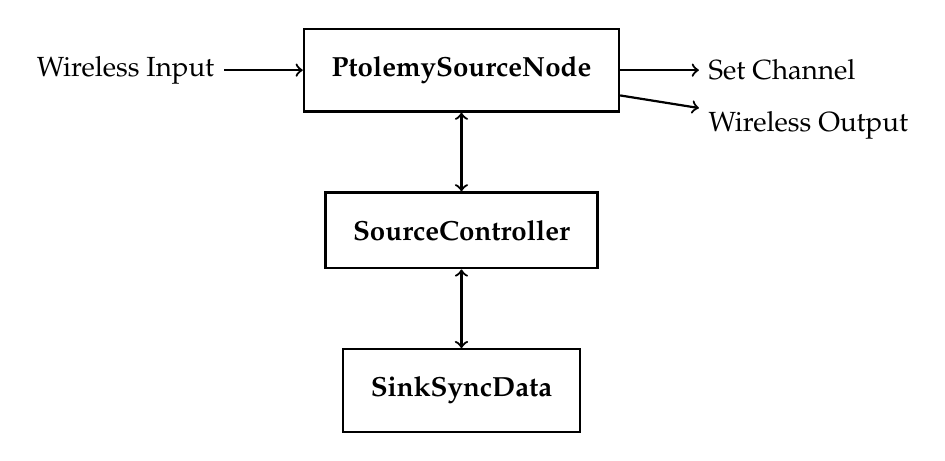
\begin{tikzpicture}[
     class/.style={draw, rectangle, thick, align=center, inner sep=1em,
		   font=\bfseries},
     port/.style={},
     arrow/.style={thick}]

    \node(SourceNode)       [class] {PtolemySourceNode};
    \node(SourceController) [class,below=of SourceNode] {SourceController}
      edge [<->,arrow] (SourceNode);
    \node(SinkSyncData)     [class,below=of SourceController] {SinkSyncData}
      edge [<->,arrow] (SourceController);

    \node(inWifi)           [port,left=of SourceNode] {Wireless Input}
      edge [->,arrow] (SourceNode);
    \node(setChannel)       [port,right=of SourceNode] {Set Channel}
      edge [<-,arrow] (SourceNode);
    \node(outWifi)          [port,below=2em of setChannel.west,anchor=west]
      {Wireless Output} edge [<-,arrow] (SourceNode);
  \end{tikzpicture}
  \caption{Exercise 1 Block Diagram}
\end{figure}

The design for the system I implemeted for Exercise 1 is split into 3 classes to
try and modularize the code and separate the different tasks:
\begin{description}
  \item[SinkSyncData]
    Controls the synchronization with one specific sink, and calculates when
    the reception period is from the data it's gathered.
  \item[SourceController]
    Coordinates multiple SinkSyncData objects (one for each sink), and
    controls which channel to listen for beacons on.
  \item[PtolemySourceNode]
    Contains the ptolemy specific code for the implementation. Most events are
    forwarded to an instance of SourceController to do any calculations.
\end{description}

\subsection{SinkSyncData}

%%%%%%%%%%%%%%%%%%%%%%% SOME INTRO HERE?

From the initial problem, it is possible to derive a function giving the exact
time each beacon frame will be received by the source.

\begin{equation*}
  f(s, n, t, i, b) = ((11 + n)i - (b - 1)t + s
\end{equation*}
\begin{description}
  \item[$s$] Absolute start time
  \item[$n$] Value of n from the protocol, number of beacons to be sent
  \item[$t$] Value of t from the protocol, time between beacons
  \item[$i$] Integer iteration number
  \item[$b$] Integer beacon number within this iteration (1 \dots $n$)
\end{description}

This function gives the absolute time a beacon occurs, but to eliminate the
value of $s$ we will subtract the times of two beacons received from a
particular sink. The function giving the time between beacons simplifies to:
\begin{align*}
  \Delta t &= f(s, n, t, i_2, b_2) - f(s, n, t, i_1, b_1) \\
           &= ((11 + n)(i_2 - i_1) - b_2 + b_1)t
\end{align*}

This is then used within the receiveBeacon function (SinkSyncData,
receiveBeacon, 78-149) to calculate good values for $n$ and $t$. By recording
the time and $n$ value of the previous beacon, we will always know the values
of $\Delta t$, $b_1$ and $b_2$. The main part of the algorithm works roughly
like this:

\begin{enumerate}
  \item Update the best $n$ value we've received so far.
  \item If we receive two beacons which are close enough to know they are
          definitely from the same iteration, we can immediately calculate
          the value of $t$ knowing that $i_2 = i_1$ and calculating
          $t = \frac{\Delta t}{b_1 - b_2}$.
\end{enumerate}

\subsection{SourceController}

\subsection{PtolemySourceNode}

- Mathematical part split into two parts
  - Data + operations related to a single Sink (SinkSyncData)
    - Calculation of n and delta t
    - Calculation of when to send the next packet (knowing n and delta t)
  - Multiple sink coordination (SourceController)
    - Owns one SinkSyncData object for each sink and demultiplexes events to
      them
    - Controls when to change channels
    - Controls when to wakeup (to send packets or for channel hopping)

- ptolemy II Model
  - Completely implemented in Java (no other ptolemy actors)
  - Wrapper around SourceController class
  - Sends events to the SourceController class
  - Obtains data and tried to set the "state of the world" to what
    SourceController wants

\section{Exercise 2 - Mote Runner}
- Code for mathemetical part is the same as the above
  - Why?
    - Code reuse - much less code to write!
    - Allows simulation in ptolemy of the ACTUAL code which will be used
    - Above code was designed to be fairly resiliant to packet loss
- Channel changing
  - Requires nothing being transmitted and the receiver must be stopped
    - Noticed some strange (undocumented) values returned by getState so I
      decided to ignore that method and use txOn and rxOn boolean variables to
      record it myself.
- SourceController does not have separate timers for things so actions are
  handled after events in a single "refresh" method handleControllerStateChange
  - Handles any previously pending transmit / receive events.
  - Attempts to transmit packets or start listening on a particular channel
  - If this failed (channel change), the event is deffered until both txOn
    and rxOn are false.

- Clock skew? (my code doesn't deal with it too much)

\end{document}
